%5_1.tex

実装した命令が正しく出力されるか,図\ref{fig:add_array_c}
に示した配列加算のプログラムを入力としてアセンブリコードの出力を行った.

\begin{figure}
    \centering
    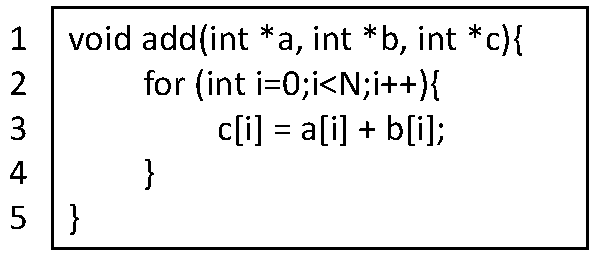
\includegraphics[scale=0.6]{image/add_array_c.pdf}
    \caption{配列加算プログラム}
    \label{fig:add_array_c}
\end{figure}

図\ref{fig:rv_vectorized_assembly}は
配列a,bの各要素の加算を配列cに格納する関数addのアセンブリコードで,データ数999個に対して一度にベクトル演算を行う配列要素を4として生成を行ったものである.25行目にあるベクトル加算のための`vadd.w'が今回実装した我々のベクトル拡張付きRISC-Vの命令である.その他の命令はRISC-Vで定義されている命令である.処理の流れはラベル`.LBB0\_2'にてベクトル演算を行っており,ラベル`LBB0\_4'にて余りの要素の処理を行っている.

\begin{figure}
    \centering
    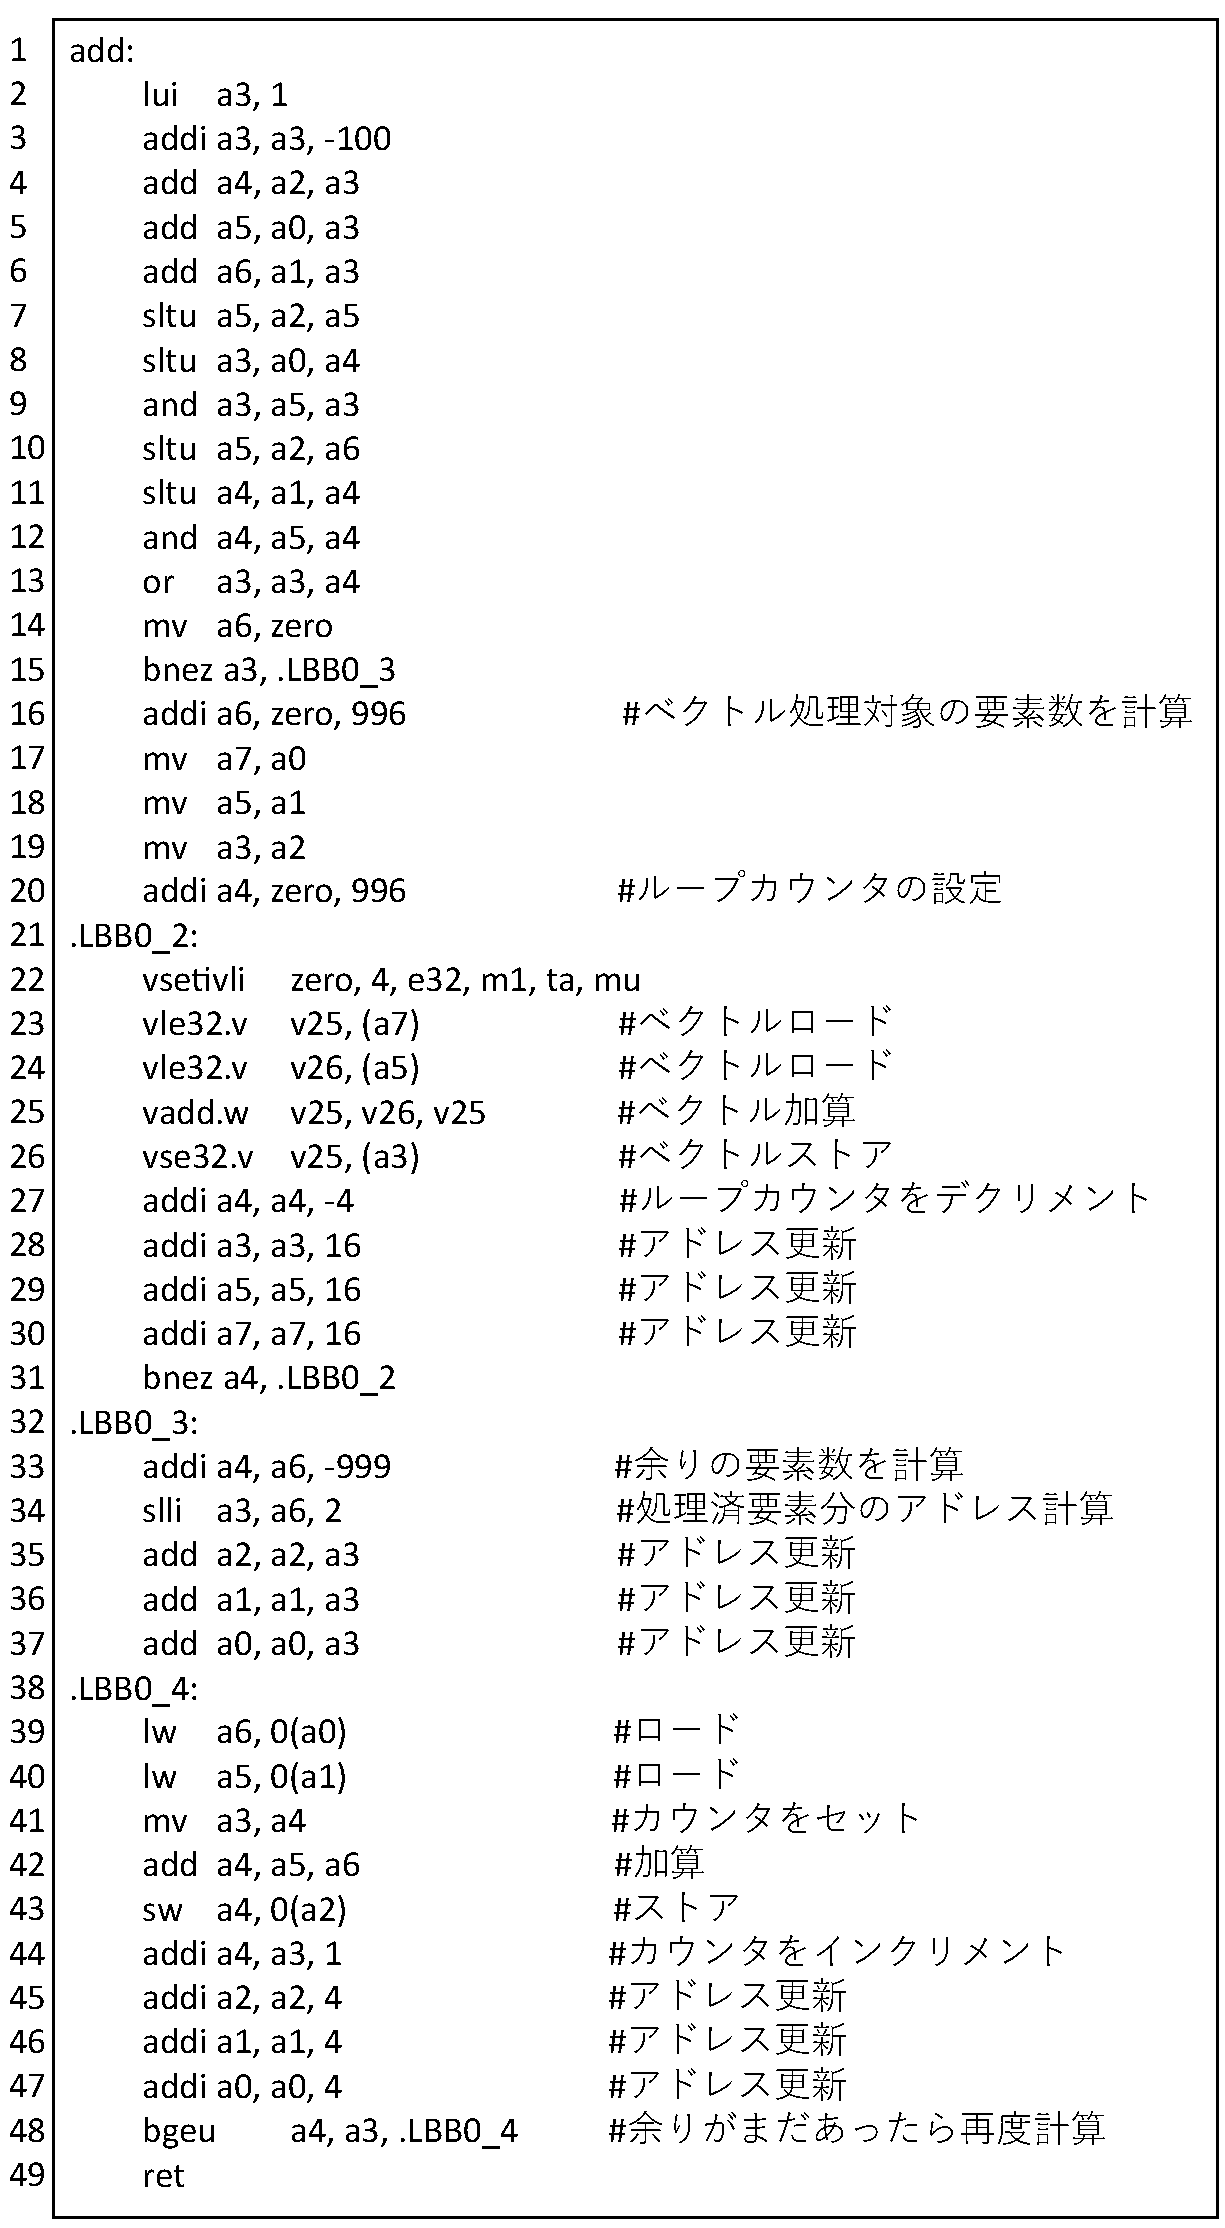
\includegraphics[scale=0.55]{image/rv_vectorized_assembly.pdf}
    \caption{生成されたアセンブリコード}
    \label{fig:rv_vectorized_assembly}
\end{figure}

図\ref{fig:add_array_c}の配列要素加算部分を変更し,他の定義した命令の生成を検証した.各命令の生成について,ベクトル処理を行っている部分を図%図番号
にまとめる.